%
\documentclass[apj]{emulateapj}
\bibliographystyle{apj}
%
\usepackage{apjfonts}
\usepackage{graphicx}
\usepackage{color}
\usepackage{amsbsy}
\usepackage{mathpazo,bm}
\usepackage{amsmath}
\usepackage{multirow}
\usepackage{natbib}
\usepackage{amssymb}
%
\newlength{\hfwidth}
\newlength{\hfwidthsingle}
\addtolength{\hfwidthsingle}{.5\textwidth} %single fig in figure
\addtolength{\hfwidth}{.497\textwidth} %single fig in figure*
%
\newcommand{\pderiv}[2]{\frac{\partial #1}{\partial #2}}
\newcommand{\pderivn}[3]{\frac{\partial^{#3} #1}{\partial #2^{#3}}}
\newcommand{\vt}[1]{\mathbf{#1}}       %for tensors
\renewcommand{\v}[1]{{\boldsymbol{#1}}} %for vectors
\def\white#1{\textcolor{white}{#1}}
\def\blue#1{\textcolor{blue}{#1}}
\definecolor{brown}{rgb}{0.42,0.24,0.07}
\def\brown#1{\textcolor{brown}{#1}}
\newcommand{\comm}[1]{({\it \brown{#1}})}
\newcommand{\del}{\v{\nabla}}
\newcommand{\grad}{\del}
\newcommand{\Div}{\del\cdot}
\newcommand{\Divp}[1]{\del\cdot\left(#1\right)}
\newcommand{\curl}{\del\times}
\newcommand{\Laplace}{\nabla^2}
%
\newcommand{\Eq}[1]{Eq. (\ref{#1})}
\newcommand{\Eqs}[2]{Eqs. (\ref{#1}) and~(\ref{#2})}
\newcommand{\Eqss}[2]{Eqs. (\ref{#1})--(\ref{#2})}
\newcommand{\eq}[1]{\Eq{#1}}
\newcommand{\eqs}[2]{\Eqs{#1}{#2}}
\newcommand{\eqss}[2]{\Eqss{#1}{#2}}
\newcommand{\eqp}[1]{(Eq. \ref{#1})}
%
\newcommand{\App}[1]{Appendix~\ref{#1}}
\newcommand{\app}[1]{\App{#1}}
\newcommand{\Figure}[1]{Figure~\ref{#1}}
\newcommand{\Fig}[1]{Fig.~\ref{#1}}
\newcommand{\fig}[1]{\Fig{#1}}
\newcommand{\Figs}[2]{Figs.~\ref{#1} and \ref{#2}}
\newcommand{\sect}[1]{Sect.~\ref{#1}}
\newcommand{\capsect}[1]{Section~\ref{#1}}
%
\newcommand{\beq}{\begin{equation}}
\newcommand{\eeq}{\end{equation}}
\newcommand{\beqn}{\begin{eqnarray}}
\newcommand{\eeqn}{\end{eqnarray}}
\newcommand{\epsp}{\varepsilon_{_{+}}}
\newcommand{\epsm}{\varepsilon_{_{-}}}

\newcommand{\St}{{\rm St}}

\shorttitle{Dust in disk vortices}
\shortauthors{Lyra \& Lin}

\slugcomment{Draft version}

\begin{document}

\title{Steady state of dust distributions in disk vortices}
\author{Wladimir Lyra\altaffilmark{1,2,3,$\star$} and Min-Kai Lin\altaffilmark{4,$\star$}}
\email{wlyra@caltech.edu, \ mklin924@cita.utoronto.ca}
\altaffiltext{1}{Jet Propulsion Laboratory, California Institute of Technology, 4800 Oak Grove Drive, Pasadena, CA, 91109, USA}
\altaffiltext{2}{Division of Geological \& Planetary Sciences, California Institute of Technology, 1200 E California Blvd MC 150-21, Pasadena, CA 91125 USA}
\altaffiltext{3}{Sagan Fellow}
\altaffiltext{4}{Canadian Institute for Theoretical Astrophysics , 60
  St. George Street, Toronto, Ontario, M5S 3H8, Canada}
\altaffiltext{$\star$}{Both authors contributed equally to this work}

\begin{abstract}
The Atacama Large Millimeter Array (ALMA) has been  returning images of transitional disks in which large asymmetries are seen in the dust distribution of 
mm-size in the outer disk. The explanation in vogue borrows from the vortex literature by suggesting 
that these asymmetries are the result of dust trapping in giant vortices, excited via Rossby wave instability (RWI) 
at planetary gap edges. Due to the drag force, dust trapped in vortices will accumulate 
in the center. Diffusion is needed to maintain a steady state over the lifetime of the disk. While previous work 
derived semi-analytical models of the process, in this paper we
provide analytical steady-steady solutions. \blue{Exact solutions exist for certain vortex models.}
The solution is determined by the vortex rotation profile, the gas scale height, the 
vortex aspect ratio, and the ratio of dust diffusion to gas-dust friction. In principle, all these quantities can be derived
from observations, which would give validation of the model, also giving constrains on the strength of the turbulence 
inside the vortex core.
\end{abstract}

\section{Introduction}
\label{sect:introduction}

Transitional disks are a class of circumstellar disks that lack a
significant near-infrared (1-5$\mu$m) excess, while showing steep
slopes in mid-infrared (5-20$\mu$m) and
far-infrared ($>$20$\mu$m) excesses typical of classical T-Tauri disks
\citep{Strom89,Skrutskie90,Gauvin-Strom92,Wolk-Walter96,Calvet02,Calvet05,Muzerolle06,Sicilia06,Currie09,Currie-Sicilia11}. 
This ``opacity hole''  implies absence of optically thick warm dust in the inner disk, with a dust
wall generating the mid-IR emission, followed by cold dust in the
outer disk.  This, together with their age (in the 1-10 Myr range, see
e.g. \citealt{Currie10} for a review) provide strong evidence that these are
objects caught in the evolutionary stage between gas-rich 
primordial and gas-poor debris disks, hence the name. 

Explanations for the opacity hole generally fall in four distinct
categories. These are, namely, grain growth and dust settling \citep{Brauer07,Dominik-Dullemond08,Zsom11,Birnstiel12}, photoevaporation
\citep{Alexander06,Cieza08,Pascucci-Sterzik09,Owen10}, 
dynamical interaction with close stellar or substellar companions
\citep{Ireland-Kraus08}, and planet
formation via dust locking \citep{Safronov69,Lyttleton72,Goldreich-Ward73,Youdin-Shu02,Johansen07} and gap
carving \citep{Papaloizou-Lin84,Lin-Papaloizou86a,Lin-Papaloizou86b,Bryden99,Paardekooper-Mellema04,Quillen04,Najita07,Andrews11}. 
Analyses of individual disks \citep{Calvet04,Calvet05,Espaillat08} tend to favor one process over another, and even census
studies of statistically significant samples of disks find one process
to be dominant \citep{Najita07,Cieza08}. These
seemingly conflicting results in fact illustrate the
heterogeneity of transitional disks, where a combination of all
suggested processes are needed to explain the rich diversity observed 
\citep{Cieza10,Muzerolle10,Merin10,Rosotti13,Clarke-Owen13}.   

Recently, high angular resolution imaging of the outer regions of transitional 
disks have become available, adding to the debate by showing a myriad of puzzling asymmetries 
that beg for explanation. These come in the shape of elliptical dust walls \citep{Isella12}, spiral arms
\citep{Muto12,Tang12}, and non-axisymmetric dust clouds \citep{Oppenheimer08,Brown09,Casassus12}. In particular, 
giant horseshoe-shaped dust distributions are seen in images obtained with \blue{the Combined Array for Research in Millimeter-wave Astronomy 
(CARMA, \citealt{Isella13})} and with the \blue{Atacama Large Millimeter Array} (ALMA, \citealt{Casassus13,vanderMarel13}). The planet interpretation is particularly attractive for 
explaining these asymmetries, since they generally match the range of structures predicted by hydrodynamical 
models of planet-disk interaction. 

A deep gap is one of these expected structures, as the planet tides expel material from the vicinity of its orbit 
\citep{Papaloizou-Lin84,Lin-Papaloizou86a,Lin-Papaloizou86b,Nelson00,Masset-Snellgrove01,Paardekooper-Mellema04,Quillen04,deValBorro06,Klahr-Kley06,Lyra09a,Zhu11,Kley12}. 
The gas gap has sharp walls, that constitute a steep pressure gradient, modifying the rotational profile locally. 
This situation is prone to excite what has been called Rossby wave
instability (RWI), that are in fact  ``edge modes'' 
\citep{Lovelace-Hohlfeld78,Toomre81,Papaloizou-Pringle84,Papaloizou-Pringle85,Hawley87,Lovelace99,Varniere-Tagger06,deValBorro07,Lyra08,Lyra09a,Lyra09b,
Meheut10,Meheut12a,Meheut12b,Meheut12c,Lin-Papaloizou11a,Lin-Papaloizou11b,Lin-Papaloizou12,Lyra-MacLow12,Lin12,Lin13} 
akin to Kelvin-Helmholtz instability, thus converting the extra shear
into vorticity. The large-scale vortices that result are well-known to trap 
dust, a property that has been invoked in the context of primordial disks to
speed up planet formation by trapping solids of cm to m size \citep{Barge-Sommeria95,Adams-Watkins95,Tanga96,Klahr-Henning97,Hodgson-Brandenburg98,Chavanis00,delaFuenteMarcos-Barge01,Johansen04,Inaba-Barge06}, and demonstrated through numerical simulations to efficiently achieve the
critical densities needed for gravitational collapse
\citep{Lyra08,Lyra09a,Lyra09b}. 

Part of these results have been applied to the field of
transitional disks. The particle size that is
preferentially trapped is set by the friction time, $\tau$, which is a
function of the gas density and particle radius. A suitable nondimensionalization for the
friction time is the Stokes number, $\St = \varOmega \tau$,
where $\varOmega$ is the Keplerian frequency. Dust that is too
well-coupled to the gas ($\St\rightarrow 0$) does not suffer friction, and bodies
that are too large ($\St\rightarrow \infty$) have too much inertia to be moved by the
gas: the preferential size for trapping is around \St=1 (see e.g. \citealt{Youdin-Goodman05,Youdin08}).
While in the dense, fast rotating, inner regions of primordial disks,
the preferentially trapped particle size corresponds to meter-size, in
the thin, slowly rotating, outer regions of transitional
disks, the size corresponding to \St=1 drops by about three orders of
magnitude \blue{\citep{Brauer07,Pinilla12a}}. The resulting trapping of sub-mm and mm-size dust may not
lead to the critical densities necessary to form planets, but they may
well explain the puzzling observed lopsided asymmetries. While the 
motivation and particle sizes are different, the relevant physics 
is scale-free, and thus identical as long as gravity is not involved. 

This property was invoked by \citet{Regaly12} to suggest that the 
sub-mm observations of \citet{Brown09} could be the result of dust
trapping in Rossby vortices. If indeed that is the case, then, 
as the drag force drives dust toward the vortex center, diffusion is
needed to maintain a steady state over the lifetime of the disk
\citep{Klahr-Henning97,Chavanis00}. \citet{Birnstiel13} presented a semi-analytical model that solves for the azimuthal dust 
distribution while using fits from numerical simulations
\citep{Pinilla12b} to constrain the radial morphology. In this work we present an analytical 
model for the steady state distribution of dust trapped in vortices, 
accurate to first order in Stokes number, and general in space. In 
\sect{sect:model-equations} we derive the
advective-diffusive equation, and in \sect{sect:coordinate-transformation} the appropriate coordinate
transformation. In \sect{sect:axisymmetric} we solve the equation for the axisymmetric
case, and in \sect{sect:nonaxisymmetric} we generalize it for non-axisymmetry. We conclude
with a brief discussion on how observations can validate the model. 

\section{Dust steady state} 
\label{sect:model-equations}

Considering the dust is of small sizes, we can treat it as a
fluid. The dust should then follow the continuity equation 

\beq
  \pderiv{\rho_d}{t} = -(\v{v}\cdot\del)\rho_d - \rho_d \Div{\v{v}} + D\Laplace{\rho_d},
  \label{eq:continuity}
\eeq

\noindent where $\rho_d$ is the dust density, $\v{v}$ is the dust
velocity, and $D$ is the diffusion coefficient (the diffusion is due
to elliptical turbulence in the vortex core and in general will be
different than the turbulent viscosity in the disk). We assume $D$ is
constant. A list of the mathematical symbols used in this work, together
with their definitions, is provided in Table~\ref{table:symbols}. 



To derive the velocities, instead of solving the momentum equations
for the dust, we make use of the relative velocity, following
\citet[see also \citealt{Youdin08}]{Youdin-Goodman05}

\beq
\v{v} = \v{u} + \tau  \grad{h}, 
\label{eq:v}
\eeq
\noindent where $\v{u}$ is the gas velocity. \eq{eq:v} is 
accurate to first order in friction time $\tau$, assumed 
constant. The enthalpy $h$ is defined as $dh = dp /\rho_g$, where $p$ 
is the pressure and $\rho_g$ the gas density. 

Inside the vortex, the gas flow is divergenceless, and 
we adopt the following model for $\v{u}$
\beq
  u_x = \varOmega_V y / \chi \qquad  u_y= -\varOmega_V x \chi,
  \label{eq:vortex}
\eeq
\noindent where $\chi > 1$ is the vortex aspect ratio (it has
semi-minor axis $a$ and semimajor axis $a\chi$). In this work
we consider the Kida solution \citep{Kida81}

\beq
\varOmega_V = \frac{3\varOmega}{2(\chi-1)},  
\eeq
which smoothly matches the above velocity field to the Keplerian
shear; as well as the GNG solution \citep{Goodman87}, that exactly solves the 
compressible Euler equations 

\beq
\varOmega_V=\varOmega\sqrt{3/(\chi^2-1)}.
\eeq

We note that the dust
velocity is comprised of a divergent-free part, $\v{u}$, and a
curl-free part, $\tau\nabla{h}$. The vortex flow attempts to keep the
dust particles on closed elliptic streamlines via $\v{u}$, while friction
attempts to concentrate dust toward pressure maximum via $\tau\nabla
h$. The only effect that attempts to spread out the dust is diffusion
via $D$.  

Taking the divergence of
\eq{eq:v} gives 

\beq
\Div{\v{v}} = \tau \Laplace{h}, 
\label{eq:divv}
\eeq

\noindent and we can find the Laplacian of the enthalpy via the Euler
equation. Adopting the shearing sheet approximation, in steady state
the force balance yields  

\begin{eqnarray}
\pderiv{h}{x} &=& 3\varOmega^2 x + 2\varOmega u_y -
u_y\pderiv{u_x}{y} \nonumber \\
&=& \left(3\varOmega^2 - 2\varOmega\varOmega_V \chi + \varOmega_V^2\right) x
= -\frac{C_1}{\tau} \  x,  \\
\pderiv{h}{y} &=& - 2\varOmega u_x -
u_x\pderiv{u_y}{x} \nonumber \\
&=& \left(-2\varOmega\varOmega_V/\chi + \varOmega_V^2\right) y = -\frac{C_2}{\tau} \  y.
\end{eqnarray}

\noindent  Substituting the equations above into \eq{eq:divv}, also
with $\omega_{_V}=\varOmega_V/\varOmega$, the divergence becomes 

\beqn
\Div{\v{v}} &=& -(C_1+C_2) = - C \label{eq:const-div}\\
&=& - \tau\varOmega^2
\left[2\omega_{_V}\left(\frac{\chi^2+1}{\chi}\right) - (2\omega_{_V}^2
  + 3) \right], 
\label{eq:scale-div}
\eeqn

\noindent where we define $C$ as positive, so that the divergence is negative (physically meaning that the dust gets trapped). Replacing \eq{eq:const-div} in the continuity equation, and setting $\partial_t$ =
0 for steady state, 

\beq
\left(D\Laplace{} -  \v{v}\cdot\del  + C\right)\rho_d = 0. 
\label{eq:steady}
\eeq

Substituting the gas velocity, and dividing by $D$, we
arrive at the modified advection-diffusion equation that should
determine the steady-state distribution of the vortex-trapped dust, 

\beq
\left[\Laplace{} - \left(Ay\chi^{-1} - B_1x\right) \partial_x  +
  \left(A x \chi + B_2y\right) \partial_y + B \right] \rho_d   = 0,  
\label{eq:dust-trapping-cartesian}
\eeq
\\
\noindent where we also substituted  $A=\varOmega_V/D$ and $B_i=C_i/D$.

\begin{table}
\caption[]{Symbols used in this work}
\label{table:symbols}
\begin{center}
\begin{tabular}{l l l}\hline
Symbol & Definition & Description \\\hline
$\tau$ && friction time\\
$\varOmega$ & & Keplerian angular frequency \\
\St & $= \varOmega \tau$ & Stokes number \\
$t$ &  & time \\
$\rho_g$, $\rho_d$  & & gas and dust density\\
$D$ & & dust diffusion coefficient \\
$\v{u}$, $\v{v}$ & & gas and dust velocity\\
$p$ && gas pressure \\
$h$ &$dh=dp/\rho_g$ & gas enthalpy\\
$\chi$ & & vortex aspect ratio ($>1$) \\
$a$ & & vortex semi-minor axis \\
$\varOmega_V$ & & vortex angular frequency \\
$\omega_{_V}$ &  $=\varOmega_V$/$\varOmega$ & dimensionless vortex frequency  \\
$C$ & $=-\Div{\v{v}}$ &  \\
$A$ & $=\varOmega_V/D$ & \\
$B$  &$=C/D$ & \\
$\nu$ & & azimuth in vortex reference frame\\
$\varepsilon_\pm$ & $ = 1\pm\chi^{-2}$ \\
$c_s$ & & sound speed \\
$H$ & $c_s/\varOmega$ & sonic scale, gas scale height\\
$\delta$ & $D=\delta c_s H$ & dimensionless diffusion parameter\\
$f(\chi)$ & \eq{eq:scale-function} & scale function \\
$H_V$ & $=\frac{H}{f(\chi)} \ \sqrt{\frac{\delta}{\St}}$ & vortex scale length \\
$k$ & $=\sqrt{2}/H_V$ & \\ 
$z$ & $=ka$ & \\
$\tilde\chi$ & $=\frac{\chi^2-1}{2(\chi^2+1)}$ & \\
%\blue{$\Delta C$} & \blue{$=(B_1-B_2)/4B$}& \\
$k_m$ & $= 1+imA/B$ & \\
$\mathcal{A}_m$ $\mathcal{B}_m$ $\mathcal{C}_m$  &\eqss{eq:ops}{eq:opsw} & differential operators \\
\blue{$b_m$} & & constants\\
$\epsilon(z)$ & & non-axisymmetric correction \\
 & & \\ \hline
\end{tabular}
\end{center}
\end{table}


\section{Change of variable}
\label{sect:coordinate-transformation}

We change variables to the coordinate system used in \citet{Chang-Oishi10}

\beqn
  x &=& a \cos\nu, \label{eq:change-x}\\
  y &=& a\chi\sin\nu.  \label{eq:change-y}
\eeqn

The system is not orthogonal, but it has the advantage of matching the
aspect ratio of the ellipses. (In contrast, the elliptic coordinate
system, though orthogonal, describes a system of confocal ellipses of
different aspect ratio, that does not coincide with the geometry of
the problem.) In these coordinates, the transformations are 

\beq
\left[\begin{array}{c}
    \partial_{a}  \\
    \partial_{\nu}
  \end{array}\right] = \vt{A} 
  \left[\begin{array}{c}
      \partial_{x}  \\
      \partial_{y}
    \end{array}\right] 
%
\quad {\rm and} \quad 
%
\left[\begin{array}{c}
    \partial_{x}  \\
    \partial_{y}
  \end{array}\right] = \vt{A}^{-1} 
  \left[\begin{array}{c}
      \partial_{a}  \\
      \partial_{\nu}
    \end{array}\right],  
%
\eeq

\noindent with 

\beq
\vt{A} = \left[\begin{array}{cc}
\pderiv{x}{a}  & \pderiv{y}{a}  \\
\pderiv{x}{\nu}  & \pderiv{y}{\nu} \\
\end{array}\right] = \left[\begin{array}{cc}
\cos\nu  & \chi\sin\nu  \\
-a\sin\nu  & a\chi\cos\nu \\
\end{array}\right]. 
\eeq

\noindent The inverse matrix is 

\beq
\vt{A}^{-1} = \frac{1}{a\chi} \left[\begin{array}{cc}
a\chi\cos\nu  & -\chi\sin\nu  \\
a\sin\nu  & \cos\nu \\
\end{array}\right].  
\eeq

The transformations are therefore

\beqn
\pderiv{}{x} &=& \cos\nu \pderiv{}{a} - \frac{\sin\nu}{a} \pderiv{}{\nu}, \\
\pderiv{}{y} &=& \frac{1}{\chi}\left(\sin\nu \pderiv{}{a} + \frac{\cos\nu}{a} \pderiv{}{\nu} \right),
\eeqn

\noindent and the Laplacian is thus 

\beqn
\Laplace{} &= &\frac{1}{2}\left[ \epsm \cos 2\nu +  \epsp\right] \partial^2_a  \nonumber \\
                &+& \frac{1}{2a^2}\left[ \epsp - \epsm \cos 2\nu\right] \partial^2_\nu \nonumber \\
                &-& \frac{\sin 2\nu}{a}\epsm \partial^2_{a\nu}   \nonumber \\
                &+& \frac{1}{2a}\left[ \epsp - \epsm \cos 2\nu\right] \partial_a \nonumber \\
                &+& \frac{\sin 2\nu}{a^2} \epsm\partial_\nu, \label{eq:laplace}
\eeqn

\noindent with $\varepsilon_{\pm} = (1 \pm \chi^{-2})$.  As for the advection term, we have 

\beqn
\v{v}\cdot\del &=& (\v{u} + \tau \grad h) \cdot \del \nonumber \\
&=& - \left[\varOmega_V - \frac{\sin2\nu}{2}  (C_1 -  C_2)\right]\partial_\nu \nonumber \\
&&- \left( C_1 \cos^2\nu   + C_2\sin^2\nu \right) a \ \partial_a. \label{eq:advection-term}
\eeqn

The dust-trapping equation is therefore 

\beqn 
&& \left\{ \Laplace{} + \left[A - \frac{\sin2\nu}{2}  (B_1 - B_2)\right]\partial_\nu \ +  \right.  \nonumber\\
&& \left. \white{\frac{1}{1}}\left( B_1 \cos^2\nu   + B_2\sin^2\nu
  \right) a \ \partial_a  + B \right\} \rho_d = 0. \label{eq:dust-trapping-uvzero}
\eeqn

\blue{We remark that a very similar equation  can be derived  when the diffusive flux is modeled as $D\rho_g\nabla(\rho_d/\rho_g)$, as used by \cite{Birnstiel13} . In fact, by redefining the friction time, 
our solution below can be made applicable to this case as well.} 

\section{``Axisymmetric'' dust distribution}
\label{sect:axisymmetric}

We now make the assumption that the dust distribution follows, in shape, that of
the gas (we will relax this approximation in the next section). In this case, the
dust distribution follows ellipses of equal aspect ratio. So,
$\partial_\nu$ = 0, ``axisymmetric'' in the ($a,\nu$)
coordinates. \eq{eq:dust-trapping-uvzero} becomes

\beqn
&&\left\{\frac{1}{2}\left(\epsm \cos 2\nu +\epsp\right) \partial^2_a  +  \left[\frac{1}{2a}\left( \epsp - \epsm\cos 2\nu\right) \right.\right. \nonumber\\
&&\left.\left.\white{\frac{1}{1}}+ (B_1\cos^2\nu +  B_2\sin^2\nu)a\right] \partial_a  + B\right\} \rho_d = 0. \label{eq:axi}
\eeqn

We now integrate the above equation in $\nu$, from 0 to 2$\pi$. This yields

\beq\label{eq:dust-trapping-axis}
\left[\partial^2_a  +  \left(\frac{1}{a} +  \frac{k^2}{2}a\right) \partial_a  + k^2\right]\rho_d = 0, 
\eeq

\noindent where we define $k^2=2B/\epsp$. Note that the parameter $A$
is absent because it represents advection by the vortex, which only
move dust particles along the same ellipse, not across it. It is
not relevant in the $\nu$-averaged problem. The solution of
\eq{eq:dust-trapping-axis} is 

\beq
\rho_d(a) = \exp\left(-\frac{k^2a^2}{4}\right)  \left[c_1 + c_2 {\rm
    Ei}\left(\frac{k^2a^2}{4}\right)\right],
\eeq

\noindent where $c_1$ and $c_2$ are constants, and ${\rm Ei}(x)$ is
the exponential integral function. Since it diverges at the origin, $c_2$ has to be zero, and 

\beq
\rho_d(a) = \rho_{d0} \exp\left(-\frac{a^2}{2H_V^2}\right),
\label{eq:gen_axi}
\eeq

\noindent with $H_V = \sqrt{2}/k$ for symmetry with the gas sonic scale. We can 
rewrite this length scale recalling that $k^2=2B/\epsp$ and
$B=C/D$. We can substitute the diffusion coefficient $D=\delta \varOmega H^2$ where 
$\delta$ is a dimensionless coefficient, and $\St = \tau\varOmega$ for 
the Stokes number, writing thus 

\beqn
\label{eq:k}
k^2 = \frac{2\St}{\delta H^2} f^2(\chi),
\eeqn 

\noindent so

\beq
 H_V = \frac{H}{f(\chi)} \sqrt{\frac{\delta}\St}. 
\label{eq:hv}
\eeq


\noindent In these equations, the scale function $f(\chi)$ is given by 

\beqn
f^2(\chi) &=& \epsp^{-1} \left[2\omega_{_V}\left(\frac{\chi^2+1}{\chi}\right) - (2\omega_{_V}^2 + 3) \right]\nonumber \\
          &=& 2\omega_{_V}\chi - \epsp^{-1}(2\omega_{_V}^2 + 3),
\label{eq:scale-function}
\eeqn

\noindent and depends on the vortex solution
used. We plot $f(\chi)$ for the Kida and GNG solutions in
\fig{fig:scale-function}. They are defined in the real axis only for $\chi > 2$ ($f^2
< 0$ for $0 < \chi < 2$ ). The Goodman solution tends to an asymptote
around 0.7. The Kida solution has a  tail around $0.5\pm0.25$ in the
interval of physical relevance ($2 < \chi \lesssim 10$). The dust distribution is thus 

\begin{figure}
  \begin{center}
    \resizebox{\columnwidth}{!}{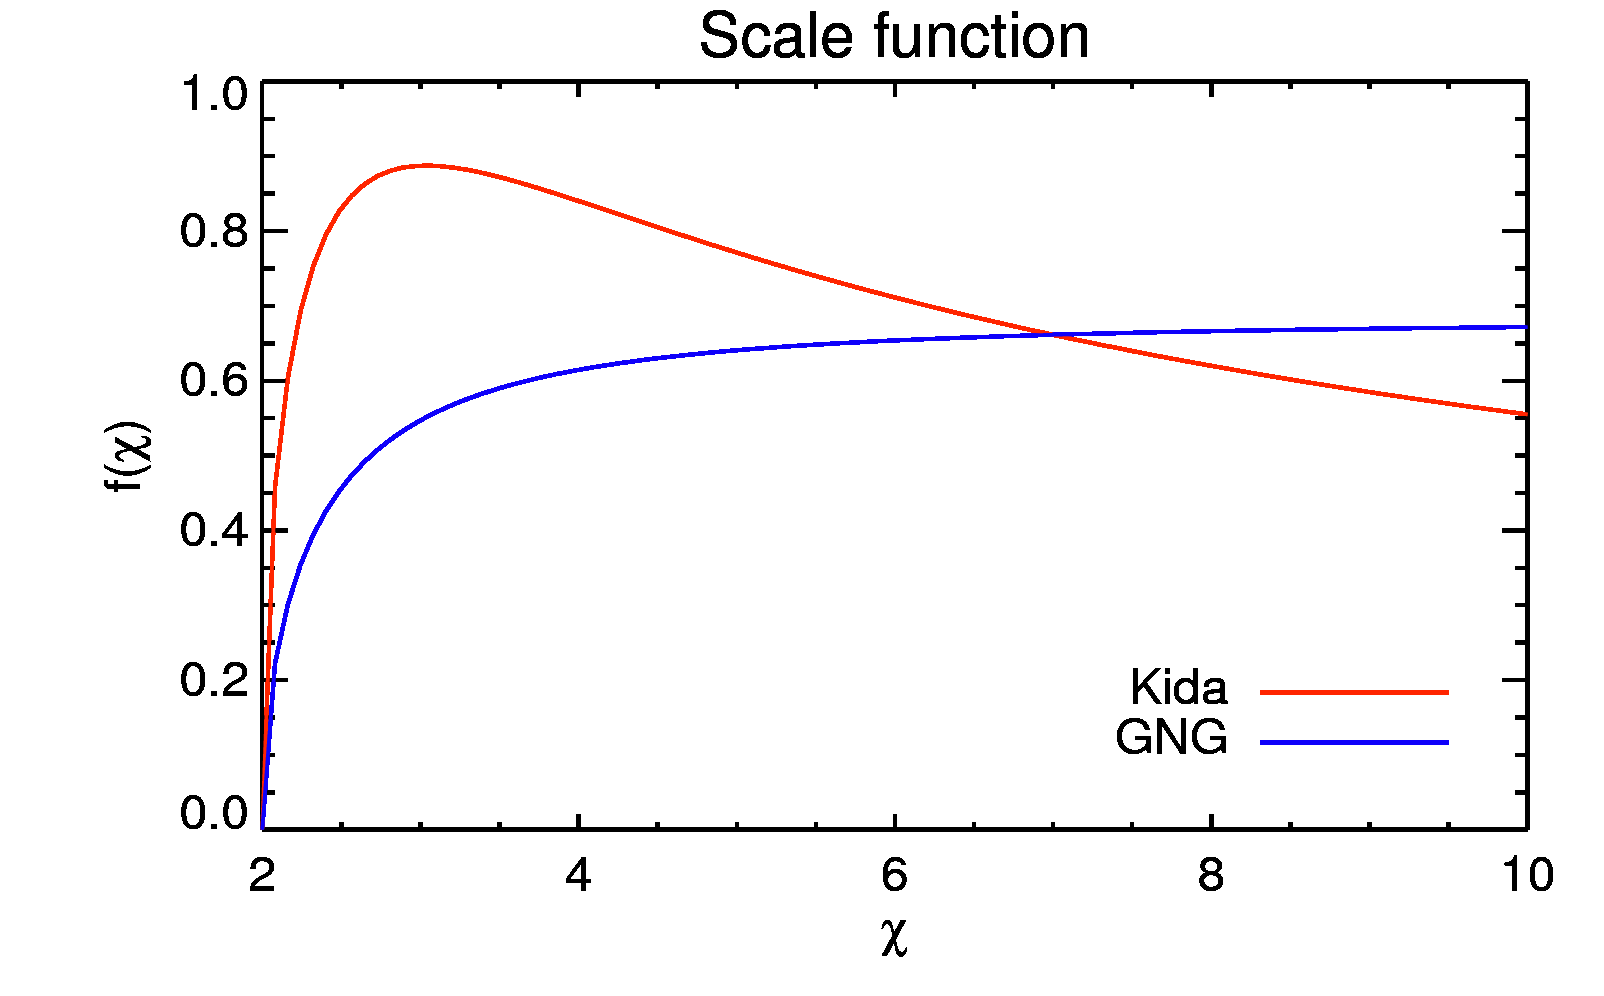
\includegraphics{../figs/scale_function.png}}
  \end{center}
\caption[]{The scale function $f(\chi)$, defined by
  \eq{eq:scale-function}, for the Kida ($\varOmega_V=3/2
  \ \varOmega_K/(\chi-1)$) and GNG ($\varOmega_V=\varOmega_K
  \sqrt{3/(\chi^2-1)}$) solutions, respectively. The scale function is
  related to the square root of the negative of the divergence
  \eqp{eq:scale-div}, and defined only for $\chi>2$. For smaller $\chi$ the
  divergence flips positive, meaning that dust is expelled from the
  vortex instead of getting trapped. This happens because of the
  correlation between $\varOmega_V$ and $\chi$. The aspect ratio shrinks
  as the vortex intensifies. At some point, the vortex rotates too
  fast, and particles are expelled by the centrifugal force.}
 \label{fig:scale-function}
\end{figure}

Dust distributions for different values of $\delta/\St$ are plotted in \fig{fig:gaussian}, as a 
function of $a/H$. We show in \fig{fig:disk}, in the inertial frame, 
the dust distribution for $\delta/\St$=1 in a Kida vortex of $\chi=4$ embedded in a 
disk of aspect ratio $H/r$=0.1, where $r$ is the stellocentric distance. 

\begin{figure}
  \begin{center}
    \resizebox{\columnwidth}{!}{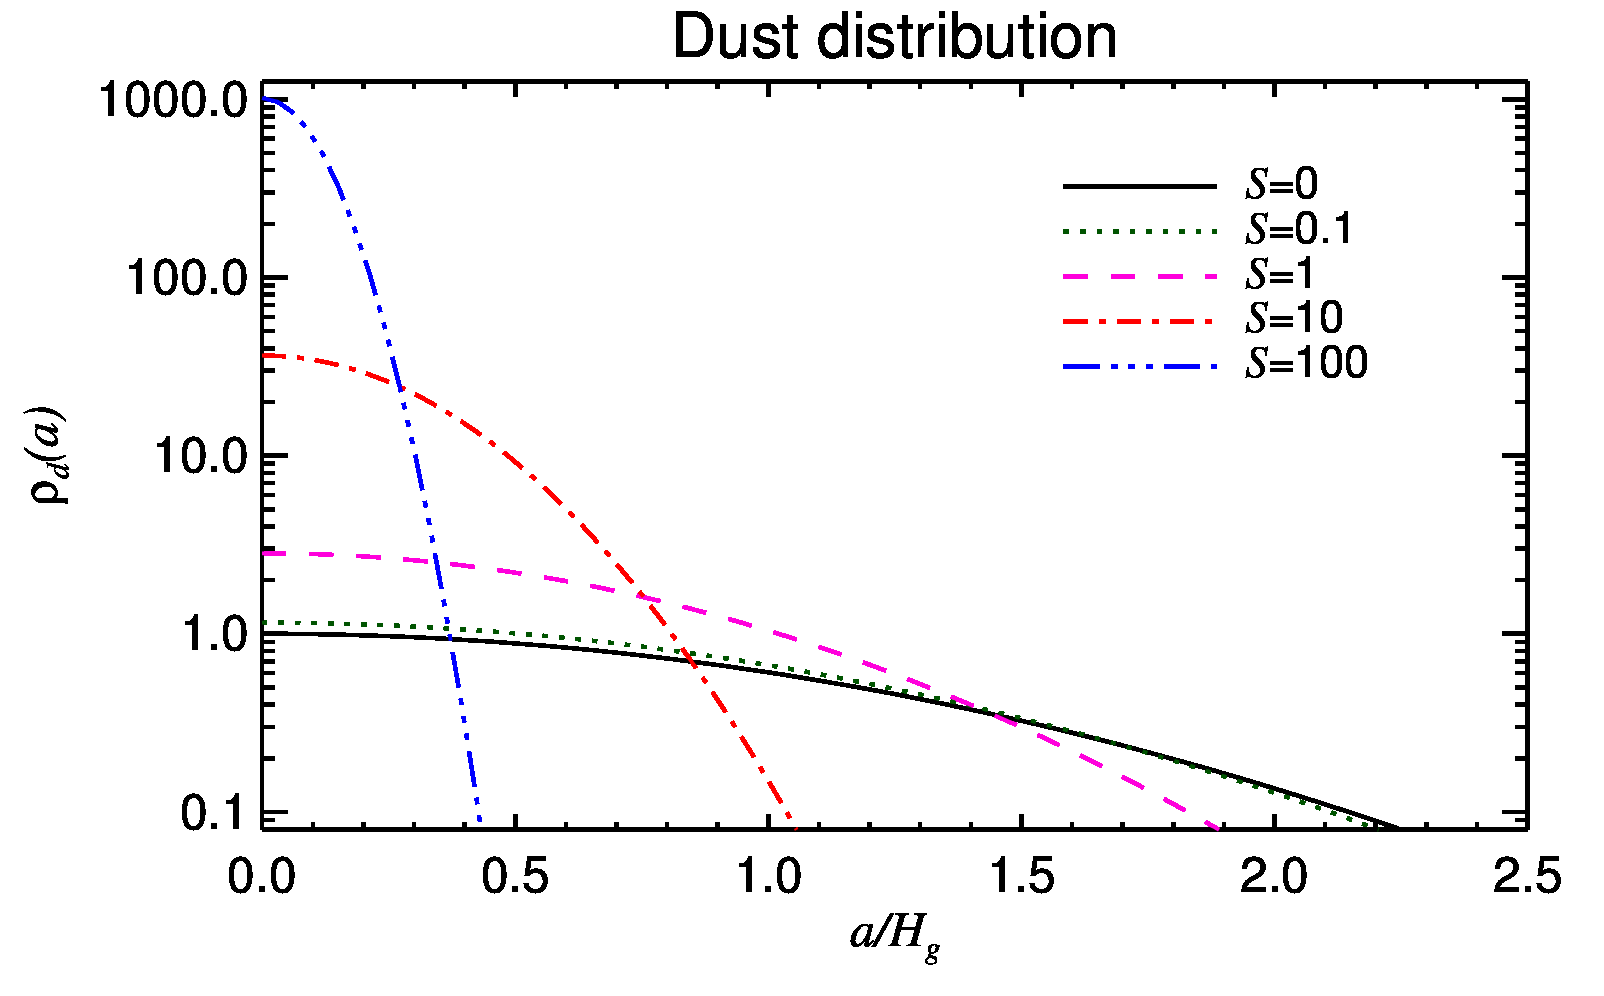
\includegraphics{../figs/gaussian.png}}
  \end{center}
\caption[]{Dust distribution for the axisymmetric case. As in
  \fig{fig:scale-function}, red and blue lines are for the Kida and
  GNG solutions, respectively. Distributions for $\delta/\St$=0.1, 1, and
  10 are shown (dashed, solid, and dot-dashed lines). The $x$-axis is
  $a/H$, where $H$ is the gas scale height. There is degeneracy
  between $\delta/\St$ and $f(\chi)$, as is clear from \eq{eq:hv}.}
 \label{fig:gaussian}
\end{figure}

\begin{figure}
\begin{center}
  \resizebox{\columnwidth}{!}{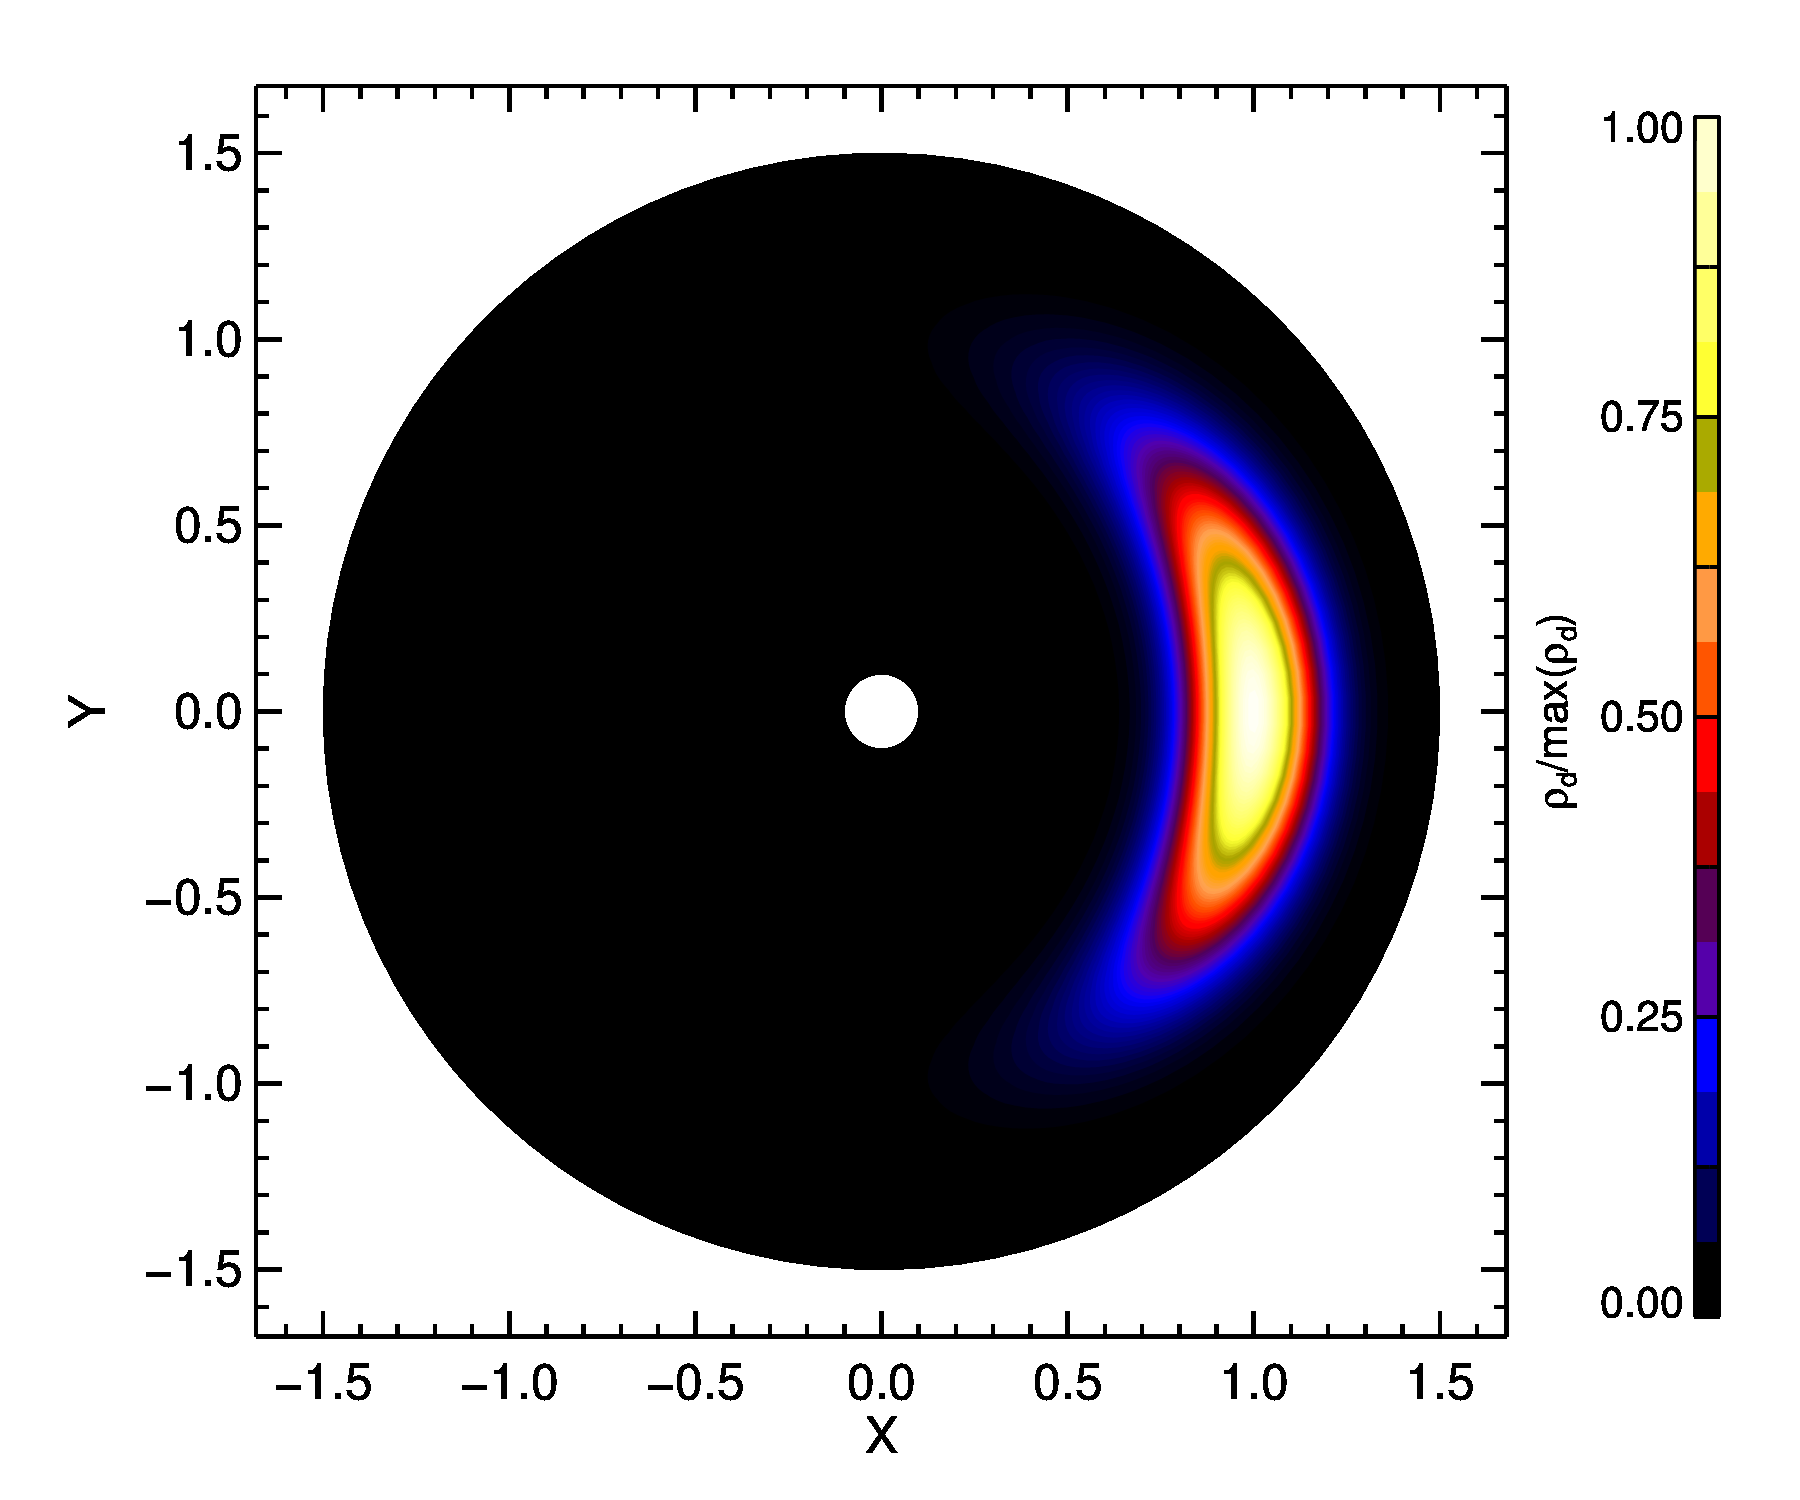
\includegraphics{../figs/disk.png}}
 \end{center}
\caption[]{Three parameters, plus a vortex solution, control the dust distribution. 
The figure shows the appearance of the dust trapped in a Kida vortex of $\chi=4$, 
for $\delta/\St$=1, in a disk of aspect ratio $H/r$=0.1.}
 \label{fig:disk}
\end{figure}

\blue{
\subsection{Exact solutions}
It is worth noting that for certain vortex models and/or aspect-ratios, the Gaussian solution, \eq{eq:gen_axi}, is in fact an exact solution to the dust-steady state equation.  We will explore this in more detail  in \sect{sect:nonaxisymmetric}, but one can check this by inserting \eq{eq:gen_axi} into \eq{eq:axi} and finding the condition for the coefficient of the trigonometric terms to vanish. In this special case, the $\nu$-integration is not needed.  
}
\subsection{Axisymmetric $\v{u} = \v{v}$ }
It is illustrative to consider the case in which $|\v{u}| \gg \tau|\grad{h}|$,
so that we can approximate $\v{v}=\v{u}$ in the advection term. (We do
not make this substitution in the compression term because $\v{u}$ is
exactly divergence-free). In this case, \eq{eq:dust-trapping-uvzero} reduces
to a relatively simple equation 

\beq\label{eq:uveq}
\left(\Laplace{} + A\partial_\nu + B \right)\rho_d = 0. 
\eeq

\eq{eq:uveq} reflects dust diffusion (first term), dust advection due
to the vortex flow (second term) and dust concentration (third term). 
Note that we are effectively considering regions close to the vortex
center because $\nabla h$ vanishes at the origin, while $\nabla^2h$
(i.e. $B$), does not.   

Now, assuming axis-symmetry and integrating in
$\frac{1}{2\pi} \int_0^{2\pi} d\nu$, we get  
\beq
\frac{\epsp}{2}\pderivn{\rho_d}{a}{2} +
\frac{\epsp}{2a}\pderiv{\rho_d}{a} + B \rho_d = 0.  
\eeq
That is, 
\beq
y^{\prime\prime} + \frac{1}{a}y^\prime + k^2 y = 0. 
\label{eq:axisymmetric}
\eeq where $y(a) = \rho_d$ and $k$ is given by \eq{eq:k}. 
\eq{eq:axisymmetric} only differs from \eq{eq:dust-trapping-axis} through the
absence of the $k^2a\partial_a$ term, which appears when the full
expression for the dust velocity is used consistently, and that term represented
axisymmetric advection, which is entirely absent in the 
problem here. Physically, as $a\to0$ there is no advection, so the two
equations behave similarly, both stating a balance between dust
concentration and dust diffusion. 

The general solution of \eq{eq:axisymmetric} is a
sum of Bessel functions of the first and second kinds: 

\beq
y(a) = c_1 J_0 (ka) + c_2 Y_0(ka). 
\eeq

\noindent Since  $Y_0$ diverges at the origin, we can physically discard 
this solution, setting $c_2=0$. So, the axisymmetric mode is $\rho_d(a)
= c_1 \ J_0 (ka)$, or

\beq
\rho_d(a) = c_1 \ J_0 \left(\frac{a}{H} \ f(\chi) \sqrt{\frac{2\St}{\delta}}\right).
\eeq 

The Bessel function $J_0(x)$ is
non-monotonic, with the first root around $x=2.5$. The first zero is therefore around
$a_0 \approx H \sqrt{\delta/\St}$.  As the density
cannot be negative, that sets the validity of our solution. 
The solution is also constrained by our use of the shearing sheet
equations, so the results should not be valid for $x \gg H$.
As we made use of the approximation $\v{v}=\v{u}$, $\St \ll 1$,
and the solution  is indeed $a_0 \gg H$, for finite values of $\delta$.

We compare in \fig{fig:bessel-gaussian} the Bessel function with the exponential found in the
previous section for the general solution. They agree up to 10\% inside
$ka$=1.5 (i.e., $a/H_V\approx 1$), and up to 1\% within $ka$=1 (i.e.,
$a/H_V\approx 0.7$). 
%Confident that approximating $\v{u}=\v{v}$ for
%advection works well within the vortex core, we use this
%simplification to find solutions to the full non-axisymmetric problem,
%in the next section. 

\begin{figure}
  \begin{center}
    \resizebox{\columnwidth}{!}{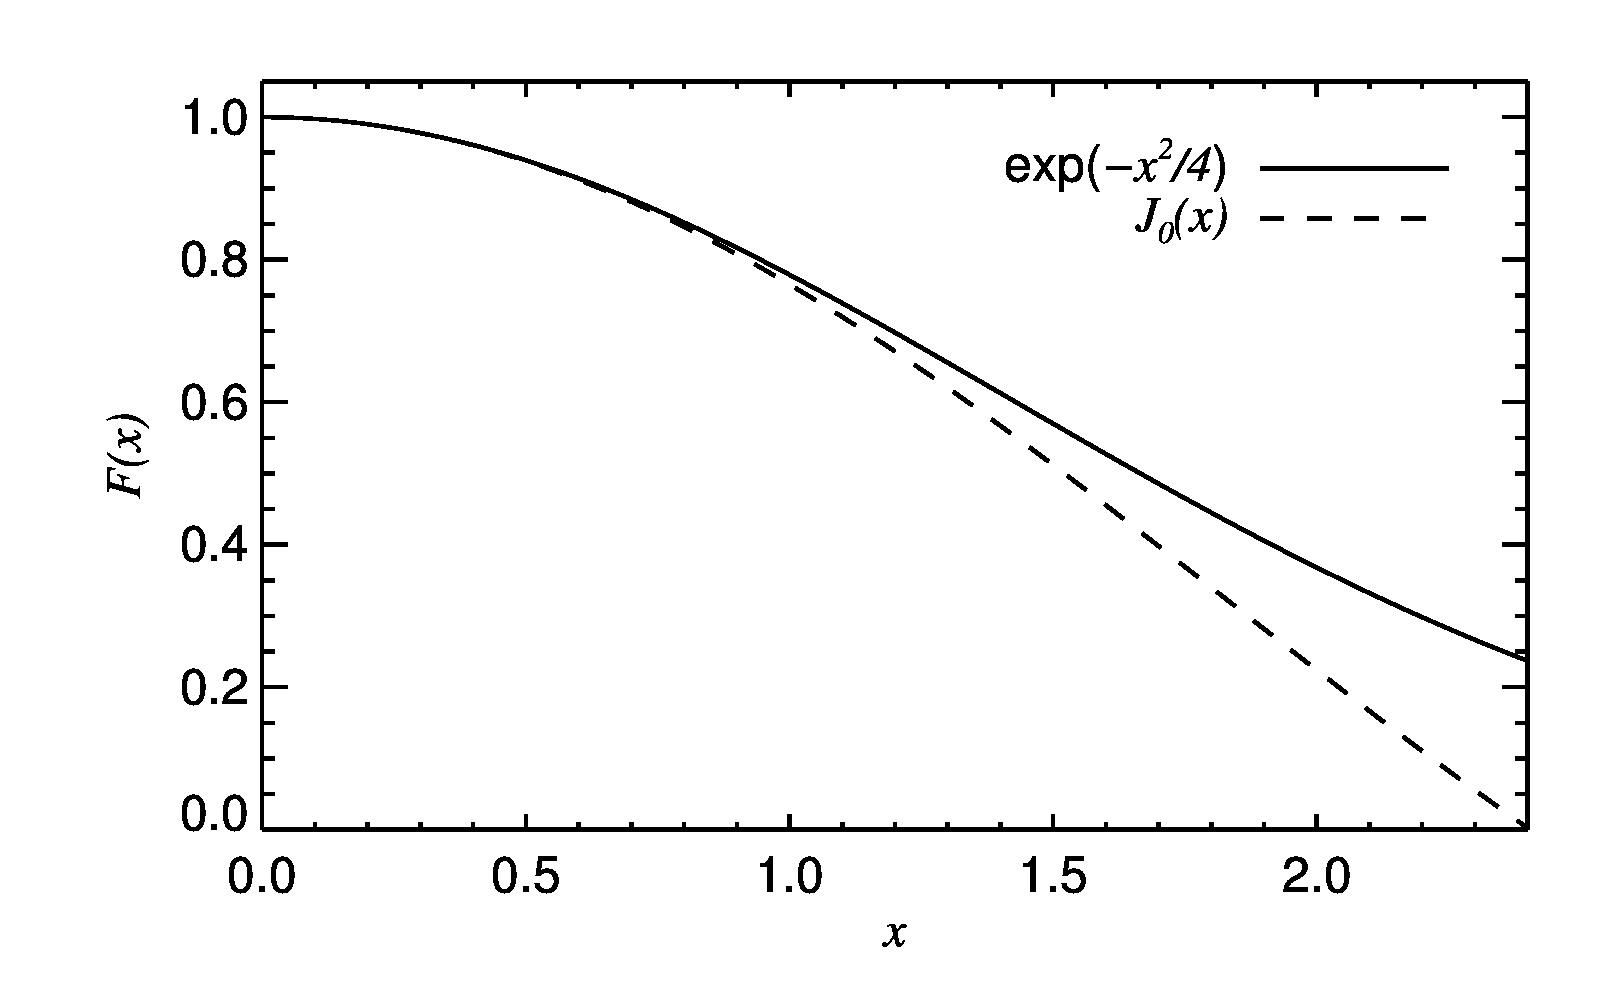
\includegraphics{../figs/bessel-gaussian.png}}
  \end{center}
\caption[]{The axisymmetric solutions for (solid line) the general 
$\v{v}=\v{u}+\tau\grad{h}$ case and, (dashed line) the case where
  we set $\v{v}=\v{u}$ for dust advection. 
The exponential and Bessel solutions agree up to 10\% up to $x$=1.5, and up 
to 1\% up to $x$=1. This means that dust advection due to $\tau\nabla{h}$
is not significant within $x\lesssim1$. We conclude that the latter
approximate solution is quite accurate for describing the dust
distribution in the vortex core.} 
 \label{fig:bessel-gaussian}
\end{figure}

\blue{
\section{Non-axisymmetric corrections}
\label{sect:nonaxisymmetric} 
}
\blue{
We now consider the non-axisymmetric problem ($\partial_\nu\neq0$). 
We explicitly show that non-axisymmetric effects are small provided the Stokes number is not 
large, and that we do not consider large distances from the vortex center. These requirements will become 
apparent as we proceed through the solution method. 
}

\blue{
\subsection{Conversion to ordinary differential equations}
We wish to solve \eq{eq:dust-trapping-uvzero}. The dust density $\rho_d$ is periodic in the $\nu$ co-ordinate. We 
therefore seek solutions of the form
\beq\label{eq:series}
\rho_d(a,\nu) = {\rm Re}
\left[\sum_{n=0}^\infty\rho_n(a)\exp{\left(\mathrm{i}n\nu\right)} \right].
\eeq
For convenience, we will drop the real part notation from now on. Inserting
\eq{eq:series} into the partial differential equation \eqp{eq:dust-trapping-uvzero},
multiplying by $\exp{(-\mathrm{i}m\nu)}$, and integrating the resulting
expressions over the $\nu$ co-ordinate, we arrive at a set of coupled
ordinary differential equations, 
}
\blue{
\beq\label{eq:ode2}
\mathcal{B}_m\rho_{m-2} (z)+ \mathcal{A}_m\rho_m(z) + \mathcal{C}_m\rho_{m+2}(z) = 0,
\eeq
}
\blue{
where $z\equiv ka$, 
\beqn
\mathcal{B}_m &\equiv& \tilde{\chi}\frac{d^2}{dz^2} + \left[\Delta C z - \frac{2\tilde{\chi}}{z}\left(m-\frac{3}{2}\right)\right]
\frac{d}{dz} \notag\\&+& \left(m-2\right)\left(\frac{m\tilde{\chi}}{z^2} -\Delta C\right),\label{eq:ops}\\
\mathcal{A}_m&\equiv&\frac{d^2}{dz^2} + \left(\frac{1}{z}+\frac{z}{2}\right)\frac{d}{dz} + \left(k_m^2-\frac{m^2}{z^2}\right),\\
\mathcal{C}_m &\equiv& \tilde{\chi}\frac{d^2}{dz^2} + \left[\Delta C z + \frac{2\tilde{\chi}}{z}\left(m+\frac{3}{2}\right)\right]
\frac{d}{dz} \notag\\&+& \left(m+2\right)\left(\frac{m\tilde{\chi}}{z^2} +\Delta C\right),\label{eq:opsw}
\eeqn
with $\tilde{\chi}\equiv(\chi^2-1)/[2(\chi^2+1)]$, $k_m^2 \equiv 1+\mathrm{i}mA/B$, and 
\begin{align}
\Delta C \equiv \frac{B_1-B_2}{2k^2(1+\chi^{-2})} = \frac{B_1 - B_2}{4B}.
\end{align}
%[Recall $k^2\equiv 2B/\left(1+\chi^{-2}\right)$.] The independent variable is $z\equiv ka$. 
Note that $\Delta C$ just depends on the vortex model. 
}

\eq{eq:ode2} holds for each $m$ except for $m=0$ for which the $\rho_{m-2}$ terms are absent. Each 
$\rho_m$ couples to $\rho_{m\pm2}$ through operators $\mathcal{B}_m$
and $\mathcal{C}_m$. The axisymmetric problem is recovered by
setting $\rho_{m>0}=0$. 

In the limit $\St\ll 1$, dust is advected by fluid with elliptic
streamlines, so we expect $\rho_d(a,\nu)$ to have even symmetry in
$\nu$. Henceforth we only consider even $m$. We seek solutions with  
$\rho_m^\prime(0)=0$ and $\rho_{m\geq2}(0)=0$, so that
$\partial_x\rho_d=\partial_y\rho_d=0$ at the origin, consistent with 
dust reaching maximal density there.  
%

\blue{
\subsubsection{Operator properties}
Consider 
\begin{align}
	g_m(z) \equiv z^m\exp{(-z^2/4)}.
\end{align}
Then we find that 
\beqn
\mathcal{B}_mg_{m-2} &=&\frac{1}{4}\left(\tilde{\chi} - 2\Delta C\right)g_m,\\
\mathcal{A}_mg_m &=& \left(k_m^2 - \frac{m}{2} - 1\right)g_m,\\
\mathcal{C}_mg_{m+2}&=& \left[4\tilde{\chi}(m+1)(m+2) +2(\Delta C-\tilde{\chi})(m+2)z^2 \right.
\notag\\ &+&\left. \frac{\left(\tilde{\chi} - 2\Delta C\right)}{4}z^4\right]g_m. 
\eeqn
The first two expressions will be useful in constructing nearly-axisymmetric solutions. 
}
\blue{
\subsection{Exactly axisymmetric solutions}
It is useful to see how the formulation above connects with the  axisymmetric solutions discussed in the previous section.  Consider the special case where $\tilde{\chi} = 2\Delta C$, so that 
%\begin{align}
$\mathcal{B}_mg_{m-2} = 0.$
%\end{align}
Then the complete solution to \eq{eq:ode2} is $\rho_0 = b_0e^{-z^2/4}$ with $\rho_{m>0} \equiv 0$, and $b_0$ is an arbitrary constant. That is, if $\tilde{\chi}=2\Delta C$ then the dust distribution is exactly axisymmetric. 
}
\blue{
\subsubsection{Dust in a GNG vortex is axisymmetric}
For the GNG vortex, one can verify that $\tilde{\chi}\equiv 2\Delta C$, implying dust density only depends on the ellipse under consideration, not the position along it. This is because the GNG vortex has no pressure gradient along the ellipctical streamlines \citep{Chang-Oishi10}. 
}
\blue{
\subsubsection{Condition for dust in a Kida vortex to be axisymmetric}
For the Keplerian Kida vortex, we find
\begin{align}
\tilde{\chi} - 2\Delta C = \frac{\chi(\chi-1)(\chi-7)}{2(\chi-2)(2\chi+1)(\chi^2+1)}.
\end{align}
The dust distribution is exactly axisymmetric for aspect-ratio $\chi=7$, which is also when the Keplerian Kida vortex has no pressure gradient along its elliptical streamlines \citep{Chang-Oishi10}. 
}
\blue{
\subsection{Source term approximation}
In preparation for constructing non-axisymmetric solutions, we here describe the \emph{source term approximation} \citep{Zhang06}.
We assume that $\rho_m$ decreases with $m$, so that in \eq{eq:ode2} the $\mathcal{C}_m\rho_{m+2}$ term has smallest magnitude.  Neglecting it as a first approximation, we solve 
}
\blue{
\begin{align}
\mathcal{A}_m\rho_m = \begin{cases}
        0 & m =0 \\
	-\mathcal{B}_m\rho_{m-2} & m \geq 2.
\end{cases}
\end{align}
The solutions are 
\begin{align}\label{eq:series}
\rho_m (z)= b_m g_m(z),
\end{align}
with
\begin{align}
b_m  = -\frac{\left(\tilde{\chi} - 2\Delta C\right)}{2\left[2k_m^2 - (m+2)\right]}b_{m-2}
\end{align}
for $m\geq2$, and $b_0$ is arbitrary as before. Note that $b_m=0$ for odd $m$ because $b_1=0$ since 
we require $\rho_1^\prime(0)=0$. Then the explicit solution is 
\begin{align}\label{eq:induction}
b_m  = \left(-1\right)^{m/2}\frac{\left(\tilde{\chi}/2-\Delta C\right)^{m/2}}{\prod_{l=1}^{m/2}
\left(2k_{2l}^2 -2l - 2\right)}b_0,
\end{align}
for even $m\geq 2$.  
}

\blue{
The source term approximation assumes 
$R\equiv|\mathcal{C}_m\rho_{m+2}|/|\mathcal{A}_m\rho_m| \ll 1.$ 
For given $z$, the solution $\rho_m=b_mg_m$ is consistent with this requirement if $|k_m^2|\gg1$, corresponding to small Stokes number.  
 However, this approximation will eventually fail for large $z$ because the solution above implies $R\propto z^4$ for $z\gg1$. Thus the solution is only self-consistent for sufficiently small $z$ and/or $\mathrm{St}$. Nevertheless,
we comment that the closed-formed solutions obtained here may be useful in
an iterative scheme to obtain numerical solutions to the full set of ODE's. 
}

\blue{
\subsection{Weakly non-axisymmetric dust distributions}
We are now ready to construct non-axisymmetric solutions. 
%The previous results indicate the axisymmetry is possible if there is no pressure gradients along the ellipse. 
Consider a Keplerian Kida vortex with $\chi\neq 7$, meaning that the frictional force on the dust has a non-vanishing component along the fluid velocity vector. (I.e. dust particles are accelerated along the ellipse.) We assume non-axisymmetry in the dust distribution is sufficiently weak, so one may truncate the series solution at $m=2$. Thus we set $\rho_{m>2}\equiv0$. 
}

\blue{
Let
\begin{align}
\rho_0(z) = b_0g_0(z) + \epsilon(z),
\end{align}
where $\epsilon(x)$ represents the correction to the axisymmetric
solution due to $\rho_2(z)$. We wish to solve
}
\blue{
\begin{align}
&\mathcal{A}_0\epsilon(z) = -\mathcal{C}_0\rho_2(z),\label{eq:m2_eq1}\\
&\mathcal{A}_2\rho_2(z)   = -\mathcal{B}_2\left(b_0g_0 + \epsilon\right).\label{eq:m2_eq2}
\end{align}
To make further progress, at this stage we \emph{assume} that the
$\epsilon$ term in Eq. \ref{eq:m2_eq2} can be neglected, so $\rho_2 = b_2 g_2$ with $b_2$ given by the source term approximation. 
This means that  
}
\blue{
\begin{align}
\frac{\rho_2}{\rho_0} = \frac{b_2}{b_0}z^2,
\end{align}
}
\blue{
implying non-axisymmetry becomes significant for sufficiently large $z$, 
and truncating the series at $m=2$ is no longer self-consistent. 
%(higher $m$ components should be included) 
However, in practice the ratio $|b_2/b_0|$ is small. 
For example, inserting $\chi=4$ gives $|b_2/b_0|\simeq0.1\%$ for $\mathrm{St}=0.1$ and $|b_2/b_0|\sim 1\%$ for $\mathrm{St}=1$. This suggests that non-axisymmetry is in general a small effect (since most of the dust is contained
within $z\lesssim 1$). 
}

\blue{
Next, we use $\rho_2 = b_2 z^2e^{-z^2/4}$ in Eq. \ref{eq:m2_eq1} to
calculate the correction term $\epsilon$. We find
}
\blue{
\begin{align}
\epsilon(z) = \frac{1}{8}b_2g_2\left[-16\tilde{\chi}+\left(\tilde{\chi} - 2\Delta C\right)z^2\right].
\end{align}
}

\blue{
Collecting the above results and Taylor-expanding the $g_m$'s, our
weakly non-axisymmetric solution for $z\ll 1$ reads:
}

\blue{
\begin{align}
&\rho_0(z) =1 -
  \frac{z^2}{4}\left[1-\frac{\tilde{\chi}\left(\tilde{\chi} - 2\Delta C\right)}{\mathrm{i}A/B - 1/2}\right]
+ O(z^4),\\
&\rho_2(z) =-\frac{\left(\tilde{\chi} - 2\Delta C\right)}{2\left(4\mathrm{i}A/B - 2\right)}z^2+O(z^4)
\end{align}
where we have used the definition of $k_m$ and set $b_0=1$ without loss of generality. We see that non-axisymmetric effects are weak for $\mathrm{St}\ll1$ because $B\propto \mathrm{St}$.  This makes sense because the force on the dust along the ellipse is proportional to $\mathrm{St}$. 
}

\blue{
\subsubsection{Consistency check}
Using the above expression for $\epsilon(z)$, we can evaluate
$\mathcal{B}_2\epsilon(z)$ in order to assess our assumption that
$\epsilon(z)$ has a negligible contribution to $\rho_2$. We find
}
\blue{
\beqn
\mathcal{B}_2\epsilon(z) =&& 
\left[32\tilde{\chi}(5\tilde{\chi} - 6\Delta C)-16(\tilde{\chi}-2\Delta C)(2\tilde{\chi}-\Delta C)z^2
\right.\notag\\&&\left.+(\tilde{\chi} - 2\Delta C)^2z^4\right]\frac{b_2g_2}{32}.
\eeqn
}
\blue{
Provided that $|k_2^2|\gg1$ and  $z$ is not large,  
this term is indeed small compared to the first term on the RHS of Eq. \ref{eq:m2_eq2}.  For example, considering $z=1$, 
for $\chi=4$ and $\mathrm{St}=0.1$ we obtain $|\mathcal{B}_2\epsilon|/|\mathcal{B}_2\rho_0|\simeq0.02$. 
Even with $\mathrm{St}=1$, this ratio $\sim0.2$ is not large. 
}

\section{Conclusions}

We solve for the distribution of dust trapped in
disk vortices, in steady state between friction, that 
tends to drive dust into the vortex, and diffusion, that expels
it. \eqs{eq:gen_axi}{eq:hv} are our result for a distribution with
``axis-symmetry''  in the coordinate system defined by
\eqs{eq:change-x}{eq:change-y}. That is, consisting of ellipses of
equal aspect ratio as those of the gas vortex. The solution has some remarkable
properties. It is a Gaussian of standard deviation $H_V$, where, given
the angular velocity $\varOmega_V$ of the vortex, $H_V$
is determined by three quantities. These are: 
the sonic length and gas scale height, $H$; the vortex aspect ratio
$\chi$; and the relative strength of diffusion to friction,
$\delta/\St$. The importance of this latter parameter had already been 
hinted upon by \citet{Cuzzi93} and \citet{Dubrulle95} 
in the context of steady states of dust sedimentation, and by
\citet{Klahr-Henning97} for vortices in the meridional plane. An insightful study by 
\citet{Jacquet12} emphasized the relevance of this parameter for 
global redistribution of solids. \citet{Birnstiel13} also find this to be 
the parameter of relevance in their semi-analytical model.

Transitional disks provide an interesting venue where to test the
model in an astrophysical context, since all three parameters can be
derivable from data. The vortex aspect ratio is readily observable,
and $H$ follows from the temperature ($H=c_s/\varOmega$). The Stokes number is a function of
dust size and internal density, as well as gas density. In principle,
these are knowable. The diffusion parameter $\delta$ is the
challenging one to quantify. In principle, it is not equal to
$\alpha$ (the dimensionless gas viscosity of
\citealt{Shakura-Sunyaev73}), because the processes generating turbulence in the
vortex and in the disk are different. The latter is supposedly the
magneto-rotational instability \citep[MRI,][]{Balbus-Hawley91}, whereas the former is the elliptic or
magneto-elliptic instability (see \citealt{Lyra13} and references
therein). A way to determine $\delta$ would be to measure the spatial rms of
the velocity field inside the vortex. The degeneracy between the
parameters ($H$, $\chi$, $\delta/\St$) and the vortex angular frequency
would also be resolved by measuring the velocity field. As these
vortices are very extended spatially, measuring their velocity field
should be possible with the exquisite angular resolution of ALMA.

We also solve for the non-axisymmetric problem, but with
approximations that render the solution valid only within 
the inner $H_V$ of distance from the vortex center. The solution is
\eq{eq:series}, with coefficients given by \eq{eq:induction}. In practice, the magnitude
of the higher non-axisymmetric modes fall fast as $m$ increases, and 
only the $m=2$ term would provide an appreciable deviation from
axisymmetry. \blue{We find that non-axisymmetry in dust 
is associated with non-zero pressure gradients along elliptical streamlines of the vortex.}

We note that, aside from planetary gap edges, self-sustained disk
vortices may also result from RWI in the boundary between MRI-active and MRI-dead zones \citep{Varniere-Tagger06,Lyra08,Lyra09a,Lyra-MacLow12}, or
convective-like nonlinear baroclinic instabilities \citep{Klahr-Bodenheimer03,Klahr04,Petersen07a,Petersen07b,Lesur-Papaloizou10,Lyra-Klahr11,Raettig13}. 
These processes, however, are not reasonable in the context of outer
regions of transition disks: the outer edge of the dead zone is quite smooth
\citep{Dzyurkevich13,Landry13}, whereas the RWI requires a 
sharp enough transition; as for the baroclinic instability, it
requires a negative radial entropy gradient, whereas the outer disk is
isothermal. This leaves gap-edge RWI as the only currently known plausible mechanism to excite such vortices. 

\acknowledgments W.L. acknowledges financial support by the National Science
Foundation under grant no. AST10-09802. Part of this paper was written
at the Jet Propulsion Laboratory, California Institute of Technology, under a contract with the
National Aeronautics and Space Administration. \blue{The authors are indebited to L. Ricci and 
J. Oishi for thoughtful suggestions.} 

\begin{thebibliography}{}
\expandafter\ifx\csname natexlab\endcsname\relax\def\natexlab#1{#1}\fi

\bibitem[{{Adams \& Watkins}(1995)}]{Adams-Watkins95} Adams, F, C. \& Watkins, R. 1995, ApJ, 451, 314
\bibitem[{{Alexander et al.}(2006)}]{Alexander06} Alexander, R. D., Clarke, C. J., \& Pringle, J. E 2006, MNRAS, 369, 216
\bibitem[{{\blue{Andrews et al.}}(2011)}]{Andrews11} \blue{Andrews, S.M., Wilner, D.J., Espaillat, C., Hughes, A.M., Dullemond, C.P., McClure, M.K., Qi, C., \& Brown, J.M. 2011, ApJ, 732, 42} 
%\bibitem[{{Artymowicz \& Lubow}(1994)}]{Artymowicz-Lubow94} Artymowicz, P. \& Lubow, S. H. 1994, ApJ, 421, 651
\bibitem[{{Balbus \& Hawley}(1991)}]{Balbus-Hawley91} Balbus, S. A. \&  Hawley, J. F. 1991, ApJ, 376, 214
\bibitem[{{Barge \& Sommeria}(1995)}]{Barge-Sommeria95} Barge, P. \&  Sommeria, J. 1995, A\&A, 295L, 1
\bibitem[{{Birnstiel et al.}(2013)}]{Birnstiel13} Birnstiel, T., Dullemond, C. P., \& Pinilla, P. 2013, A\&A, 550L, 8
\bibitem[{{\blue{Birnstiel et al.}}(2012)}]{Birnstiel12} \blue{Birnstiel, T., Andrews, S. M., \& Ercolano, B. 2012, A\&A, 544, 79}
\bibitem[{{Brauer et al.}(2007)}]{Brauer07} Brauer, F., Dullemond, C.P., \blue{Johansen, A.,} Henning, Th.\blue{, Klahr, H., \& Natta, A.} 2007, A\&A, 469, 1169
\bibitem[{{Brown et al.}(2009)}]{Brown09} Brown, J. M., Blake, G. A., Qi, C., Dullemond, C. P., Wilner, D. J., \& Williams, J. P. 2009, ApJ, 704, 496
\bibitem[{{Bryden et al.}(1999)}]{Bryden99} Bryden, G., Chen, X., Lin, D. N. C., Nelson, R. P., \& Papaloizou, J. C. B. 1999, ApJ, 514, 344
\bibitem[{{Calvet et al.}(2002)}]{Calvet02} Calvet, N., D'Alessio, P., Hartmann, L., Wilner, D., Walsh, A., \& Sitko, M. 2002, ApJ, 568, 1008
\bibitem[{{Calvet et al.}(2004)}]{Calvet04} Calvet, N., Muzerolle, J., Brice\~no, C.,  Hern\'andez, J., Hartmann, L., Saucedo, J.L., \& Gordon, K.D. 2004, AJ, 128, 1294
\bibitem[{{Calvet et al.}(2005)}]{Calvet05} Calvet, N., D'Alessio, P., Watson, D. M., Franco-Hern\'andez, R., Furlan, E., Green, J., Sutter, P. M., Forrest, W. J., Hartmann, L., Uchida, K. I., Keller, L. D.,Sargent, B., Najita, J., Herter, T. L., Barry, D. J., \& Hall, P. 2005, ApJ, 630, 185
\bibitem[{{Casassus et al.}(2012)}]{Casassus12} Casassus, S., Perez M., S., Jord\'an, A., M\'enard, F., Cuadra, J., Schreiber, M. R., Hales, A. S., \& Ercolano, B. 2012, ApJ, 754, 31
\bibitem[{{Casassus et al.}(2013)}]{Casassus13} Casassus, S., van der Plas, G., Perez, S., Dent, W.R.F., Fomalont, E., Hagelberg, J., Hales, A., Jord\'an, A., Mawet, D., M\'enard, F., Wootten, A., Wilner, D., Hughes, M., Schreiber, M.R., Girard, J.H., Ercolano, B., Canovas, H., Rom\'an, P., \& Salinas, V. 2013, Nature, 493, 191
%\bibitem[{{Chandrasekhar}(1960)}]{Chandrasekhar60} Chandrasekhar, S., 1960, Proc. Nat. Acad. Sci., 46, 253
%\bibitem[{{Chandrasekhar}(1961)}]{Chandrasekhar61} Chandrasekhar 1961 {\it Hydrodynamic and Hydromagnetic Stability} (Oxford: Clarendon), 384
\bibitem[{{Chang \& Oishi}(2010)}]{Chang-Oishi10} Chang, P. \& Oishi, J.S. 2010, ApJ, 721, 1593
\bibitem[{{Chavanis}(2000)}]{Chavanis00} Chavanis, P.-H. 2000, A\&A, 356, 1089
\bibitem[{{Cieza}(2008)}]{Cieza08} Cieza, L.A., Swift, J.J., Mathews, G.S., \& Williams, J.P. 2008, ApJ, 686, 115
\bibitem[{{Cieza}(2010)}]{Cieza10} Cieza, L.A., Schreiber, M.R., Romero, G.A., Mora, M.D., Mer\'in, B., Swift, J.J., Orellana, M., Williams, J.P., Harvey, P.M., \& Evans, N.J. 2010, ApJ, 712, 925
\bibitem[{{Clarke \& Owen}(2013)}]{Clarke-Owen13} Clarke, C.J. \& Owen, J.E. 2013, MNRAS, accepted, arXiv:1305.2483
\bibitem[{{Currie et al.}(2009)}]{Currie09} Currie, Th., Lada, C.J., Plavchan, P.,  Robitaille, T.P., Irwin, J., \& Kenyon, S.J. 2009, ApJ, 698, 1
\bibitem[{{Currie}(2010)}]{Currie10} Currie, Th. 2010, arXiv1002.1715C	
\bibitem[{{Currie \& Sicilia-Aguilar}(2011)}]{Currie-Sicilia11} Currie, Th. \& Sicilia-Aguilar, A. 2011, ApJ, 732, 24
\bibitem[{{Cuzzi et al.}(1993)}]{Cuzzi93} Cuzzi, J.N., Dobrovolskis, A.R., \& Champney, J.M. 1993, Icarus, 106, 102
\bibitem[{{Dominik \& Dullemond}(2008)}]{Dominik-Dullemond08} Dominik, C. \& Dullemond, C. P. 2008, A\&A, 491, 663
\bibitem[{{Dubrulle et al.}(1995)}]{Dubrulle95} Dubrulle, B., Morfill, G., \& Sterzik, M. 1995, Icarus, 114, 237
\bibitem[{{Dzyurkevich et al.}(2013)}]{Dzyurkevich13} Dzyurkevich, N., Turner, N.J., Henning, Th., \& Kley, W. 2013, ApJ, 765, 114
\bibitem[{{Espaillat et al.}(2008)}]{Espaillat08} Espaillat, C., Calvet, N., Luhman, K.L., Muzerolle, J., \& D'Alessio, P. 2008, ApJ, 682L, 125
%\bibitem[{{Espaillat et al.}(2010)}]{Espaillat10} Espaillat, C., D'Alessio, P., Hern\'andez, J., Nagel, E., Luhman, K. L., Watson, D. M., Calvet, N., Muzerolle, J., \& McClure, M. 2010, ApJ, 717, 441
\bibitem[{{de la Fuente Marcos \& Barge}(2001)}]{delaFuenteMarcos-Barge01} de la Fuente Marcos, C. \& Barge, P. 2001, MNRAS, 323, 601 
\bibitem[{{Gauvin \& Strom}(1992)}]{Gauvin-Strom92} Gauvin, L.S. \& Strom, K.M. 1992, ApJ, 385, 217
\bibitem[{{Goldreich \& Ward}(1973)}]{Goldreich-Ward73} Goldreich, P. \& Ward, W.R. 1973, ApJ, 183, 1051
\bibitem[{{Goodman et al.}(1987)}]{Goodman87} Goodman, J., Narayan, R., \& Goldreich, P. 1987, MNRAS, 225, 695
\bibitem[{{Hawley}(1987)}]{Hawley87} Hawley, J.F. 1987, MNRAS, 225, 677
%\bibitem[{{Hawley et al.}(1995)}]{Hawley95} Hawley, J.F., Gammie, C.F., \& Balbus, S.A. 1995, ApJ, 440, 742
\bibitem[{{Lovelace \& Hohlfeld}(1978)}]{Lovelace-Hohlfeld78}  Lovelace, R.V.E. \& Hohlfeld, R.G. 1978, ApJ, 221, 51
\bibitem[{{Hodgson \& Brandenburg}(1998)}]{Hodgson-Brandenburg98} Hodgson, L.S. \& Brandenburg A. 1998, A\&A, 330, 1169
%\bibitem[{{Huelamo et al.}(2011)}]{Huelamo11} Hu\'elamo, N., Lacour, S., Tuthill, P., Ireland, M.,  Kraus, A., \& Chauvin, G. 2011, A\&A, 528L, 7
\bibitem[{{Inaba \& Barge}(2006)}]{Inaba-Barge06} Inaba, S. \& Barge, P. 2006, ApJ, 649, 415
\bibitem[{{Ireland \& Kraus}(2008)}]{Ireland-Kraus08} Ireland, M. J. \& Kraus, A. L. 2008, ApJ, 678L, 59
\bibitem[{{\blue{Isella et al.}}(2013)}]{Isella13} \blue{Isella, A., P\'erez, L.M., Carpenter, J.M., Ricci, L., Andrews, S., \& Rosenfeld, K. 2013, ApJ, submitted}
\bibitem[{{Isella et al.}(2012)}]{Isella12} Isella, A., P\'erez, L.M., \& Carpenter, J.M. 2012, ApJ, 747, 136
\bibitem[{{Johansen et al.}(2004)}]{Johansen04} Johansen, A., Andersen, A. C., \& Brandenburg, A. 2004, 417, 361
\bibitem[{{Johansen et al.}(2007)}]{Johansen07} Johansen, A., Oishi, J. S., Mac Low, M.-M., Klahr, H., Henning, Th., \& Youdin, A. 2007, Nature, 448, 1022
\bibitem[{{Kida}(1981)}]{Kida81} Kida, S. 1981, J. Phys. Soc. Jpn.,  50, 351
\bibitem[{{Klahr}(2004)}]{Klahr04} Klahr, H. 2004, ApJ, 606, 1070
\bibitem[{{Klahr \& Bodenheimer}(2003)}]{Klahr-Bodenheimer03} Klahr, H. \& Bodenheimer, P. 2003, ApJ, 582, 869
\bibitem[{{Klahr \& Henning}(1997)}]{Klahr-Henning97} Klahr, H.H. \& Henning, Th. 1997, Icarus, 128, 213
\bibitem[{{Klahr \& Kley}(2006)}]{Klahr-Kley06} Klahr, H. \& Kley, W. 2006, A\&A, 445, 747
\bibitem[{{Kley et al.}(2012)}]{Kley12} Kley, W., M\"uller, T. W. A., Kolb, S. M., Ben\'itez-Llambay, P., \& Masset, F. 2012, A\&A, 546, 99
%\bibitem[{{Kraus \& Ireland}(2012)}]{Kraus-Ireland12} Kraus, AL. \& Ireland, M.J. 2012, ApJ, 745, 5
\bibitem[{{Jacquet et al.}(2012)}]{Jacquet12} Jacquet, E., Gounelle, M., \& Fromang, S. 2012, Icarus, 220, 162
\bibitem[{{Landry et al.}(2013)}]{Landry13} Landry, R., Dodson-Robinson, S.E., Turner, N.J., \& Abram, G. 2013, arXiv1305.0770
\bibitem[{{Lin \& Papaloizou}(1986a)}]{Lin-Papaloizou86a} Lin, D.N.C. \& Papaloizou, J. 1986a, ApJ, 307, 395
\bibitem[{{Lin \& Papaloizou}(1986b)}]{Lin-Papaloizou86b} Lin, D.N.C. \& Papaloizou, J. 1986b, ApJ, 309, 846
\bibitem[{{Lin \& Papaloizou}(2011a)}]{Lin-Papaloizou11a} Lin, M.-K. \& Papaloizou, J.C.B. 2011, MNRAS, 415, 1426
\bibitem[{{Lin \& Papaloizou}(2011b)}]{Lin-Papaloizou11b} Lin, M.-K. \& Papaloizou, J.C.B. 2011, MNRAS, 415, 1445
\bibitem[{{Lin \& Papaloizou}(2012)}]{Lin-Papaloizou12} Lin, M.-K. \& Papaloizou, J.C.B. 2012, MNRAS, 421, 780
\bibitem[{{Lin}(2012)}]{Lin12} Lin, M.-K. 2012, ApJ, 754, 21
\bibitem[{{Lin}(2013)}]{Lin13} Lin, M.-K. 2013, ApJ, 765, 84
\bibitem[{{Lesur \& Papaloizou}(2010)}]{Lesur-Papaloizou10} Lesur, G. \& Papaloizou, J.C.B. 2010, A\&A, 513, 60
\bibitem[{{Lovelace et al.}(1999)}]{Lovelace99} Lovelace, R.V.E., Li, H., Colgate, S.A., \& Nelson, A. F. 1999, ApJ, 513, 805
\bibitem[{{Lyra}(2013)}]{Lyra13} Lyra, W. 2013, in {\it Instabilities and Structures in Proto-Planetary Disks}, Marseille, France, Edited by P. Barge; L. Jorda; EPJ Web of Conferences, Volume 46, id.04003 
\bibitem[{{Lyra \& Mac Low}(2012)}]{Lyra-MacLow12} Lyra, W. \& Mac Low, M.-M. 2012, ApJ, 756, 62
\bibitem[{{Lyra \& Klahr}(2011)}]{Lyra-Klahr11} Lyra, W. \& Klahr,  H. 2011, A\&A, 527A, 138
\bibitem[{{Lyra et al.}(2009b)}]{Lyra09b} Lyra, W., Johansen, A., Zsom, A., Klahr, H., Piskunov, N. 2009b, A\&A, 497, 869
\bibitem[{{Lyra et al.}(2009a)}]{Lyra09a} Lyra, W., Johansen, A., Klahr, H., Piskunov, N. 2009a, A\&A, 493, 1125 
\bibitem[{{Lyra et al.}(2008)}]{Lyra08} Lyra, W., Johansen, A., Klahr, H., \& Piskunov, N. 2008, A\&A, 491, L41
\bibitem[{{Lyttleton}(1972)}]{Lyttleton72} Lyttleton, R.A. 1972, MNRAS, 160, 255
\bibitem[{{van der Marel et al.}(2013)}]{vanderMarel13} van der Marel et al. 2013, Science, accepted
\bibitem[{{Masset \& Snellgrove}(2001)}]{Masset-Snellgrove01} Masset, F. \& Snellgrove, M. 2001, MNRAS, 320L, 55
\bibitem[{{M\'eheut et al.}(2010)}]{Meheut10} M\'eheut, H., Casse, F., Varni\`ere, P., \& Tagger M. 2010, A\&A, 516, 31
\bibitem[{{M\'eheut et al.}(2012a)}]{Meheut12a} M\'eheut H., Cong, Y., \& Lai, D. 2012, MNRAS, 422, 2399
\bibitem[{{M\'eheut et al.}(2012b)}]{Meheut12b} M\'eheut H., Keppens,  R., Casse, F., \& Benz, W. 2012, A\&A, 542A, 9
\bibitem[{{M\'eheut et al.}(2012c)}]{Meheut12c} M\'eheut, H., Meliani, Z., Varni\`ere, P., \& Benz, W. 2012, A\&A, 545, 134
\bibitem[{{Mer\'in et al.}(2010)}]{Merin10} Mer\'in, B., Brown, J. M., Oliveira, I., Herczeg, G.J., van Dishoeck, E.F., Bottinelli, S., Evans, N.J., Cieza, L., Spezzi, L., Alcal\'a, J.M., Harvey, P.M., Blake, G.A., Bayo, A., Geers, V.G., Lahuis, F., Prusti, T., Augereau, J.-C., Olofsson, J., Walter, F.M., \& Chiu, K. 2010, ApJ, 718, 1200
\bibitem[{{Muto et al.}(2012)}]{Muto12} Muto, T., Grady, C. A., Hashimoto, J., Fukagawa, M., Hornbeck, J. B. et al. 2012, ApJ, 748L, 22
\bibitem[{{Muzerolle et al.}(2006)}]{Muzerolle06} Muzerolle, J., Adame, L., D'Alessio, P., Calvet, N., Luhman, K.L., Muench, A.A., Lada, C.J., Rieke, G.H., Siegler, N., Trilling, D.E., Young, E.T., Allen, L., Hartmann, L., \& Megeath, Th. 2006, ApJ, 643, 1003
\bibitem[{{Muzerolle et al.}(2010)}]{Muzerolle10} Muzerolle, J., Allen, L.E., Megeath, Th., Hern\'andez, J., \& Gutermuth, R.A. 2010, ApJ, 708, 1107
\bibitem[{{Najita et al.}(2007)}]{Najita07} Najita, J.R., Strom, S.E., \& Muzerolle, J. 2007, MNRAS, 378, 369
\bibitem[{{Nelson et al.}(2000)}]{Nelson00} Nelson, R.P., Papaloizou, J.C.B., Masset, F., \& Kley, W. 2000, MNRAS, 318, 18
%\bibitem[{{Olofsson et al.}(2011)}]{Olofsson11} Olofsson, J., Benisty, M., Augereau, J.-C., Pinte, C., M\'enard, F., Tatulli, E., Berger, J.-P., Malbet, F., Mer\'in, B., van Dishoeck, E.F., Lacour, S., Pontoppidan, K.M., Monin, J.-L., Brown, J.M., \& Blake, G.A. 2011, A\&A, 528L, 6O
\bibitem[{{Oppenheimer et al.}(2008)}]{Oppenheimer08} Oppenheimer, B.R., Brenner, D., Hinkley, S., Zimmerman, N., Sivaramakrishnan, A., Soummer, R., Kuhn, J., Graham, J.R., Perrin, M., Lloyd, J.P., Roberts, L.C., \& Harrington, D.M. 2008, ApJ, 679, 1574
\bibitem[{{Owen et al.}(2010)}]{Owen10} Owen, J.E., Ercolano, B., Clarke, C.J., \& Alexander, R.D. 2010, MNRAS, 401, 1415
\bibitem[{{Paardekooper \& Mellema}(2004)}]{Paardekooper-Mellema04} Paardekooper, S.-J. \& Mellema, G.	2004, A\&A, 425L, 9
\bibitem[{{Papaloizou \& Lin}(1984)}]{Papaloizou-Lin84} Papaloizou, J. \& Lin, D.N.C. 1984, ApJ, 285, 818
\bibitem[{{Papaloizou \& Pringle}(1984)}]{Papaloizou-Pringle84} Papaloizou, J.C.B. \& Pringle, J.E. 1984, MNRAS, 208, 721
\bibitem[{{Papaloizou \& Pringle}(1985)}]{Papaloizou-Pringle85} Papaloizou, J.C.B. \& Pringle, J.E. 1985, MNRAS, 213, 799
\bibitem[{{Pascucci \& Sterzik}(2009)}]{Pascucci-Sterzik09} Pascucci, I. \& Sterzik, M. 2009, ApJ, 702, 724
\bibitem[{{Petersen et al.}(2007a)}]{Petersen07a} Petersen, M. R., Julien, K., Stewart, G. R. 2007a, ApJ, 658, 1236
\bibitem[{{Petersen et al.}(2007b)}]{Petersen07b} Petersen, M. R., Stewart, G. R., Julien, K. 2007b, ApJ, 658, 1252
\bibitem[{{Pinilla et al.}(2012b)}]{Pinilla12b} Pinilla, P., Benisty, M., \& Birnstiel, T. 2012\blue{b}, A\&A, 545, 81
\bibitem[{{\blue{Pinilla et al.}}(2012a)}]{Pinilla12a} \blue{Pinilla, P., Birnstiel, T., Ricci, L., Dullemond, C.P., Uribe, A.L., Testi, L., \& Natta, A. 2012a, A\&A, 538, 114} 
%\bibitem[{{Pott et al.}(2010)}]{Pott10} Pott, J.-U., Perrin, M.D., Furlan, E., Ghez, A.M., Herbst, T.M., \& Metchev, S. 2010, ApJ, 710, 265
\bibitem[{{Quillen et al.}(2004)}]{Quillen04} Quillen, A.C., Blackman, E.G., Frank, A., \& Varni\`ere, P. 2004, ApJ, 612, 137
\bibitem[{{Raettig et al.}(2013)}]{Raettig13} Raettig, N., Lyra, W., \& Klahr, H. 2013, ApJ, 765, 115
\bibitem[{{Reg\'aly et al.}(2012)}]{Regaly12} Reg\'aly, Zs., Juh\'asz, A., S\'andor, Zs, \& Dullemond, C.P. 2012, MNRAS, 419, 1701
\bibitem[{{\blue{Rosotti et al.}}(2013)}]{Rosotti13} \blue{Rosotti, G.P., Ercolano, B., Owen, J.E., \& Armitage, P.J. 2013, MNRAS, 430, 1392} 
\bibitem[{{Safronov}(1969)}]{Safronov69} Safronov, V. S. 1969, Evoliutsiia Doplanetnogo Oblaka (English transl: Evolution of the Protoplanetary Cloud and Formation of Earth and the Planets, NASA Tech. Trans. F-677, Jerusalem: Israel Sci. Transl., 1972)
\bibitem[{{Sicilia-Aguilar et al.}(2006)}]{Sicilia06} Sicilia-Aguilar, A., Hartmann, L.W., F\"ur\'esz, G., Henning, Th., Dullemond, C., \& Brandner, W. 2006, AJ, 132, 2135
\bibitem[{{Shakura \& Sunyaev}(1973)}]{Shakura-Sunyaev73} Shakura, N. I. \& Sunyaev, R. A. 1973, A\&A, 24, 337
\bibitem[{{Skrutskie et al.}(1990)}]{Skrutskie90} Skrutskie, M. F., Dutkevitch, D., Strom, S.E., Edwards, S., Strom, K.M., \& Shure, M.A. 1990, AJ, 99, 1187
\bibitem[{{Strom et al.}(1989)}]{Strom89} Strom, K.M., Strom, S.E., Edwards, S., Cabrit, S., \& Skrutskie, M.F. 1989, AJ, 97, 1451
\bibitem[{{\blue{Tang et al.}}(2012)}]{Tang12} \blue{Tang, Y.-W., Guilloteau, S., Pi\'etu, V., Dutrey, A., Ohashi, N., \& Ho, P.T.P. 2012, A\&A, 547, 84}
\bibitem[{{Tanga et al.}(1996)}]{Tanga96} Tanga P., Babiano, A., Dubrulle, B., \& Provenzale, A. 1996, Icarus, 121, 158
\bibitem[{{Toomre}(1981)}]{Toomre81} Toomre, A. 1981, What amplifies the spirals. In {\it The Structure and Evolution of Normal Galaxies}, Proceedings of the Advanced Study Institute, Cambridge, England, Cambridge and New York, Cambridge University Press, 1981, p.111-136.
%\bibitem[{{Umurhan}(2010)}]{Umurhan10} Umurhan O. M. 2010, A\&A, 521,  25
\bibitem[{{de Val-Borro et al.}(2007)}]{deValBorro07}de Val-Borro, M., Artymowicz, P., D'Angelo, G., Peplinski, A. 2007, A\&A, 471, 1043
\bibitem[{{de Val-Borro et al.}(2006)}]{deValBorro06}de Val-Borro, M., Edgar, R.G., Artymowicz, P., Ciecielag, P., Cresswell, P., D'Angelo, G., Delgado-Donate, E.J., Dirksen, G., Fromang, S., Gawryszczak, A., Klahr, H., Kley, W., Lyra, W., Masset, F., Mellema, G., Nelson, R., Paardekooper, S.-J., Peplinski, A., Pierens, A., Plewa, T., Rice, K., Sch\"afer, C., \& Speith, R. 2006, MNRAS
\bibitem[{{Varni\`ere \& Tagger}(2006)}]{Varniere-Tagger06} Varni\`ere, P. \& Tagger, M. 2006, A\&A, 446, 13
%\bibitem[{{Velikhov}(1959)}]{Velikhov59} Velikhov, E. P. 1959, Soviet Phys. JETP, 36, 1398
\bibitem[{{Wolk \& Walter}(1996)}]{Wolk-Walter96} Wolk, S.J. \& Walter, F.M. 1996, AJ, 111, 2066
\bibitem[{{Youdin \& Goodman}(2005)}]{Youdin-Goodman05} Youdin, A. N. \& Goodman, J. 2005, ApJ, 620, 459
\bibitem[{{Youdin \& Shu}(2002)}]{Youdin-Shu02} Youdin, A. N. \& Shu, F. H. 2002, ApJ, 580, 494
\bibitem[{{Youdin}(2008)}]{Youdin08} Youdin, A. 2008arXiv:0807.1114
\blue{\bibitem[Zhang \& Lai(2006)]{Zhang06} Zhang, H., \& Lai, D.\ 2006, MNRAS, 368, 917}
\bibitem[{{Zhu et al.}(2011)}]{Zhu11} Zhu, Zh., Nelson, R.P., Hartmann, L.,  Espaillat, C., \& Calvet, N. 2011, ApJ, 729, 47
\bibitem[{{Zsom et al.}(2011)}]{Zsom11} Zsom, A., Ormel, C.W., Dullemond, C.P., \& Henning, Th. 2011, A\&A, 534, 73
\end{thebibliography}

\end{document}
